\documentclass{standalone}

\usepackage{pgf,tikz}
\usepackage{pgfplots}
\usepackage[europeanresistors,americaninductors]{circuitikz}
\usetikzlibrary{spy}
\begin{document}
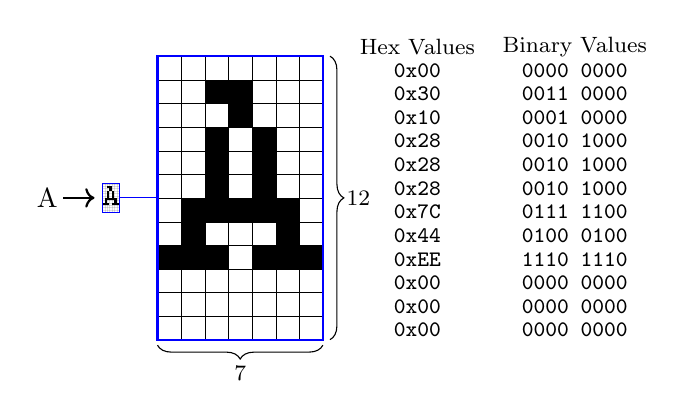
\begin{tikzpicture}
 [line cap=round,line join=round,x=1cm,y=1cm,
spy using outlines={rectangle,lens={scale=10}, height = 3.6cm, width = 2.1cm, connect spies},
%using the decoration 'brace' (=a curly brace as path replacement)
decoration={brace,amplitude=2pt}]
\node[anchor=center] at (-1.7, 6.08) {A};

\draw [decorate,decoration={brace,amplitude=5pt,mirror,raise=4pt},yshift=0pt]
(-0.3,4.35) -- (1.8,4.35) node [black,midway,yshift=-0.5cm] {\footnotesize
	$7$};

\draw [decorate,decoration={brace,amplitude=5pt,mirror,raise=4pt},yshift=0pt]
(1.75,4.28) -- (1.75,7.88) node [black,midway,xshift=0.5cm] {\footnotesize
	$12$};
\node[anchor=center] at (3, 8) {\footnotesize Hex Values};
\node[anchor=center] at (3, 7.7) {\footnotesize \texttt{0x00}};
\node[anchor=center] at (3, 7.4) {\footnotesize \texttt{0x30}};
\node[anchor=center] at (3, 7.1) {\footnotesize \texttt{0x10}};
\node[anchor=center] at (3, 6.8) {\footnotesize \texttt{0x28}};
\node[anchor=center] at (3, 6.5) {\footnotesize \texttt{0x28}};
\node[anchor=center] at (3, 6.2) {\footnotesize \texttt{0x28}};
\node[anchor=center] at (3, 5.9) {\footnotesize \texttt{0x7C}};
\node[anchor=center] at (3, 5.6) {\footnotesize \texttt{0x44}};
\node[anchor=center] at (3, 5.3) {\footnotesize \texttt{0xEE}};
\node[anchor=center] at (3, 5 ) {\footnotesize  \texttt{0x00}};
\node[anchor=center] at (3, 4.7) {\footnotesize \texttt{0x00}};
\node[anchor=center] at (3, 4.4) {\footnotesize \texttt{0x00}};


\node[anchor=center] at (5, 8) {\footnotesize Binary Values};
\node[anchor=center] at (5, 7.7) {\footnotesize \texttt{0000 0000}};
\node[anchor=center] at (5, 7.4) {\footnotesize \texttt{0011 0000}};
\node[anchor=center] at (5, 7.1) {\footnotesize \texttt{0001 0000}};
\node[anchor=center] at (5, 6.8) {\footnotesize \texttt{0010 1000}};
\node[anchor=center] at (5, 6.5) {\footnotesize \texttt{0010 1000}};
\node[anchor=center] at (5, 6.2) {\footnotesize \texttt{0010 1000}};
\node[anchor=center] at (5, 5.9) {\footnotesize \texttt{0111 1100}};
\node[anchor=center] at (5, 5.6) {\footnotesize \texttt{0100 0100}};
\node[anchor=center] at (5, 5.3) {\footnotesize \texttt{1110 1110}};
\node[anchor=center] at (5, 5 ) {\footnotesize  \texttt{0000 0000}};
\node[anchor=center] at (5, 4.7) {\footnotesize \texttt{0000 0000}};
\node[anchor=center] at (5, 4.4) {\footnotesize \texttt{0000 0000}};


\draw[thick, ->](-1.5,6.08)->(-1.1,6.08);
  \begin{scope}
%\draw [step=0.03,very thin] (-1, 5.9) grid (-0.79, 6.26);

\foreach \i in {-1,-0.97,...,-0.79}
{
	\draw [line width=0.001mm](\i, 5.9) -- (\i, 6.26);
}
\foreach \i in {5.9,5.93,...,6.26}
{
	\draw [line width=0.001mm](-1, \i) -- (-0.79, \i);
}

\fill [black] (-1, 5.99) rectangle (-0.91, 6.02);
\fill [black] (-0.88, 5.99) rectangle (-0.79, 6.02);
\fill [black] (-0.97, 6.02) rectangle (-0.94, 6.05);
\fill [black] (-0.85, 6.02) rectangle (-0.82, 6.05);
\fill [black] (-0.97, 6.05) rectangle (-0.82, 6.08);
\fill [black] (-0.94, 6.08) rectangle (-0.91, 6.17);
\fill [black] (-0.85, 6.08) rectangle (-0.88, 6.17);
\fill [black] (-0.88, 6.17) rectangle (-0.91, 6.20);
\fill [black] (-0.88, 6.20) rectangle (-0.94, 6.23);



\spy [blue] on (-0.895,6.08)
				in node [left] at (1.8,6.08);
%\node[anchor=center] at (3, -0.5) {Font size 12 Description 7 Pixel wide 12 High};
\end{scope}


\end{tikzpicture}
\end{document}
